\documentclass[landscape, hidelinks,10pt]{article}

% BODY TEXT
\usepackage[utf8]{inputenc}
\usepackage[english]{babel}

\usepackage{geometry}
\geometry{a4paper,margin=2cm}

\usepackage{multicol}
\setlength{\columnsep}{1cm}


% COMPACT LIST
\newenvironment{myitemize}
{ \begin{itemize}
	\setlength{\itemsep}{2pt}
	\setlength{\parskip}{0pt}
	\setlength{\parsep}{0pt}     }
{ \end{itemize}                  }

% CODE SNIPPETS
\usepackage{xcolor}
\usepackage{minted}

% URLs
\usepackage{hyperref}

% MATH
\usepackage{amssymb}

% OTHER

\usepackage{graphicx}


\setlength{\parskip}{0.5em}
\setlength{\parindent}{0em}


\begin{document}

\begin{multicols*}{2}


\title{Software Carpentry Python\\Summary Document}
\author{Blair Wang\\hello@blair.wang}

\maketitle

\par
This document is written to summarise (and, in some cases, extend) the ``Programming with Python'' Software Carpentry course. Each of the twelve parts of that course are summarised in this document in one A4 page.

\par
The original materials for that Software Carpentry course can be found online at \url{https://swcarpentry.github.io/python-novice-inflammation/}. The source code for this document can be found online at \url{https://github.com/blairw/swcpythonsummary}.

\par
Both the original materials and this summary document are licensed under Creative Commons Attribution 4.0 International (CC BY 4.0).

\columnbreak
\tableofcontents

\end{multicols*}

\raggedright
\section{Python Fundamentals}
\begin{multicols*}{2}
\subsection{Variables}
\par
To start with, we can think of Python as a calculator so you can do a calculation like ``3 + 5 × 4'':

\vspace{-4mm}
\begin{minted}[xleftmargin=6mm,frame=lines,framesep=2mm,linenos]{python}
>>> 3 + 5 * 4
23
\end{minted}

\par
The above is what it looks like in an interactive Python shell (\mintinline{zsh}{python3} at a bash/zsh shell). However, if you are running a Python \textit{script} (e.g. \mintinline{zsh}{python3 myscript.py}), you will not see anything. In that latter case, you will need to type into your Python script:

\vspace{-4mm}
\begin{minted}[xleftmargin=6mm,frame=lines,framesep=2mm,linenos]{python}
print(3 + 5 * 4)
\end{minted}

\par
Like any good `scientific' calculator, you can also store the results of calculations into variables like how you can do \texttt{Ans $\rightarrow$ A}. However, unlike your typical high school scientific calculator, Python gives you much more flexibility in naming your variables. Therefore, you should give your variables meaningful names. \mintinline{python}{A} would actually be a very bad name for a variable in most cases. Your variables should be named according to the business context, e.g. if we were writing some Python script about the Consumer Price Index (CPI):

\vspace{-4mm}
\begin{minted}[xleftmargin=6mm,frame=lines,framesep=2mm,linenos]{python}
cpi_june_2019 = 0.6
print(cpi_june_2019)
\end{minted}

\subsection{Data Types}
You will notice in the above we first worked with \textbf{integers} ($\mathbb{Z}$, e.g. 1, 2, 3) and then there was an example with a \textbf{rational number} ($\mathbb{Q}$, e.g. 0.6, $\frac{1}{3}$). Rational numbers are stored in Python as so-called ``floating-point'' numbers or ``floats''. Floats can sometimes behave strangely:

\vspace{-4mm}
\begin{minted}[xleftmargin=6mm,frame=lines,framesep=2mm,linenos]{python}
>>> 1.1 + 1.3
2.4000000000000004
\end{minted}

To cope with this, we can use \textbf{libraries}. A library is some additional component of Python that gives us access to additional programming functionality, e.g.:

\vspace{-4mm}
\begin{minted}[xleftmargin=6mm,frame=lines,framesep=2mm,linenos]{python}
>>> from fractions import Fraction
>>> from decimal import Decimal
>>>
>>> Decimal(1.1) + Decimal(1.3)
Decimal('2.400000000000000133226762955')
>>> # this ^ is still the wrong answer
>>> # we should enclose the numbers in quotes
>>> 
>>> Decimal('1.1') + Decimal('1.3')
Decimal('2.4')
>>> # correct answer! :)
>>>
>>> Fraction(1,3) + Fraction(1,3)
Fraction(2, 3)
>>> print(Fraction(1,3) + Fraction(1,3))
2/3
>>> print(float(Fraction(1,3) + Fraction(1,3)))
0.6666666666666666
\end{minted}

You may notice in the above that I have used the ``hash'' symbol to make \textbf{comments}. This is very useful for explaining your code.

\subsection{Additional Tips}
\begin{myitemize}
\item If you want to, you can assign multiple variables at the same time, e.g. \mintinline{python}{mass, age = 25.5, 20}. Only do this if it makes your code more readable.
\item In additional to the numerical data types discussed above, Python also has the data type for text strings (e.g. the classic: \mintinline{python}{print('Hello world')}). You can use either single quotes or double quotes. This can be useful in some situations, e.g.  \mintinline{python}{print('In French: "Bonjour tout le monde"')}.
\item Variable names can include letters, digits and underscores. However, they cannot \textit{begin} with a digit. For example, you cannot create a variable called  \mintinline{python}{12th_person}.
\end{myitemize}


\end{multicols*}
\section{Analyzing Patient Data}
\begin{multicols*}{2}
\subsection{Loading the ``Inflammation'' CSV Files}
\par
The Software Carpentry Python course involves a very simple case study involve a set of CSV (comma-separated values) data files. CSV files are simply text files where each line of text is a new role and each line is formatted like \texttt{0.5,52.2,12.1} (hence \textit{comma-separated} values). In our ``Inflammation'' case study, which is from a medical context, each row is an arthritis patient and each column is a day of data about the severity of inflammation that these patients are experiencing.
\par
Because this is a CSV file that is all numerical, we can use the numbers library for Python (\texttt{numpy}):

\vspace{-4mm}
\begin{minted}[xleftmargin=6mm,frame=lines,framesep=2mm,linenos]{python}
import numpy as np
data = np.loadtxt(fname='inflammation-01.csv', delimiter=',')
print(data.shape) # returns (60, 40) = 60 rows, 40 columns
\end{minted}

\par
Please note that this will not work unless you have numpy installed. I recommend doing this using a virtual environment (venv):

\vspace{-4mm}
\begin{minted}[xleftmargin=6mm,frame=lines,framesep=2mm,linenos]{bash}
python3 -m venv .venv          # create the venv
source .venv/bin/activate      # activate the venv
python3 -m pip install numpy   # install numpy inside the venv
python3                        # do stuff in Python
deactivate                     # deactivate the venv when done
\end{minted}

\subsection{Getting Data Points and Ranges}
\begin{myitemize}
    \item Arrays in Python are indexed from 0. This means that, for example, that what we would usually call the ``first'' column is, in Python, column ``0''; the ``second'' column is column ``1'', etc.
    \item You can get a data point (``cell'' in spreadsheet terminology) by \textbf{specifying coordinates as ``row, column''}. For example, what we might think of in Microsoft Excel as cell ``C5'' (= ``fifth row, third column'' = row ``4'', column ``2'' in Python) can be obtained like so:
\vspace{-2mm}
\begin{minted}[xleftmargin=6mm,frame=lines,framesep=2mm,linenos]{python}
data_c5 = data[4, 2]
\end{minted}
    \item You can get a range by specifying the starting point and that which is \textit{after} the ending point. This could be quite intuitive in the sense that \mintinline{python}{data[0:4, 0:10]} means ``first 4 rows, first 10 columns'', but since you can specify ranges that don't start from 0, it could also take some more mental arithmetic to be sure what you're doing (e.g. \mintinline{python}{data[5:8, 3:15]} = rows 5 to 7 (0-indexed), columns 3 to 14 (0-indexed)).
    \item You can also have unbounded ranges, e.g. \mintinline{python}{data[ :8, 3: ]} = all rows up to and including row 7, all rows including and after column 3.

\end{myitemize}

\subsection{Descriptive Statistics}
Given a numpy array, you can print the usual descriptive statistics:

\vspace{-4mm}
\begin{minted}[xleftmargin=6mm,frame=lines,framesep=2mm,linenos]{python}
print('minimum inflammation:', np.min(data))
print('maximum inflammation:', np.max(data))
print('mean:', np.mean(data))
print('standard deviation:', np.std(data))
\end{minted}

Each of those operations (min, max, mean, std) returns a signle value. However, you could also generate an array of values. For example, maybe you want a list of the mean inflammation scores for each patient (i.e., mean across rows); or you might want a list of mean inflammation scores for each day (i.e., mean across columns).

To do this, we specify a value for \texttt{axis}:

\vspace{-4mm}
\begin{minted}[xleftmargin=6mm,frame=lines,framesep=2mm,linenos]{python}
avg_across_days = numpy.mean(data, axis=0)
avg_for_each_patient = numpy.mean(data, axis=1)
\end{minted}

You basically just have to remember that \textbf{``axis 0'' means columns and ``axis 1'' means rows}, even though coordinates are specified as ``row, column''.

\end{multicols*}
\section{Visualizing Tabular Data}
\begin{multicols*}{2}

The Software Carpentry Python course suggests using the \mintinline{python}{matplotlib} library for charts and graphs. This is a decent library for simple charts and graphs, though for anything more sophisticated you might want to look into \mintinline{python}{seaborn}.

\textbf{Important Reminder:} Just like with \texttt{numpy}, you will have to install \texttt{matplotlib} before proceeding:

\vspace{-4mm}
\begin{minted}[xleftmargin=6mm,frame=lines,framesep=2mm,linenos]{bash}
deactivate && source .venv/bin/activate
python3 -m pip install matplotlib
\end{minted}

\subsection{Heatmap with \texttt{imshow}}

Assuming we still have \mintinline{python}{data} set up as the CSV numpy array from the previous section, we can generate a heatmap simply with:

\vspace{-4mm}
\begin{minted}[xleftmargin=6mm,frame=lines,framesep=2mm,linenos]{python}
import matplotlib.pyplot
image = matplotlib.pyplot.imshow(data)
matplotlib.pyplot.savefig('imshow_output.png')
matplotlib.pyplot.show()
\end{minted}

Note that the line 4 only works if you are running Python in a graphical environment: it shows a pop-up with the graphic. \textbf{This is not the case if you are running Python in a Linux shell inside WSL 1.} In that situation, you can remove line 4 and just use the \mintinline{bash}{imshow_output.png} file generated in line 3.

\subsection{Graphing with \texttt{plot}}

The \texttt{matplotlib} library also draws simple line graphs. For example, recalling that each column in this dataset is a day's worth of data, \textbf{``axis 0'' means columns}, we could graph the trend of the daily average inflammation:

\vspace{-4mm}
\begin{minted}[xleftmargin=6mm,frame=lines,framesep=2mm,linenos]{python}
ave_inflammation = numpy.mean(data, axis=0)
ave_plot = matplotlib.pyplot.plot(ave_inflammation)
matplotlib.pyplot.savefig('plot_output.png')
\end{minted}

\subsection{Drawing a \texttt{figure}}
\label{ch3_figure}

\par
You might recall some rules about proper charts and graphs: you should always include a title; you should always label the axes. You may also wish to combine multiple charts and graphs into a single picture. All the above can be achieved using \texttt{figure}.

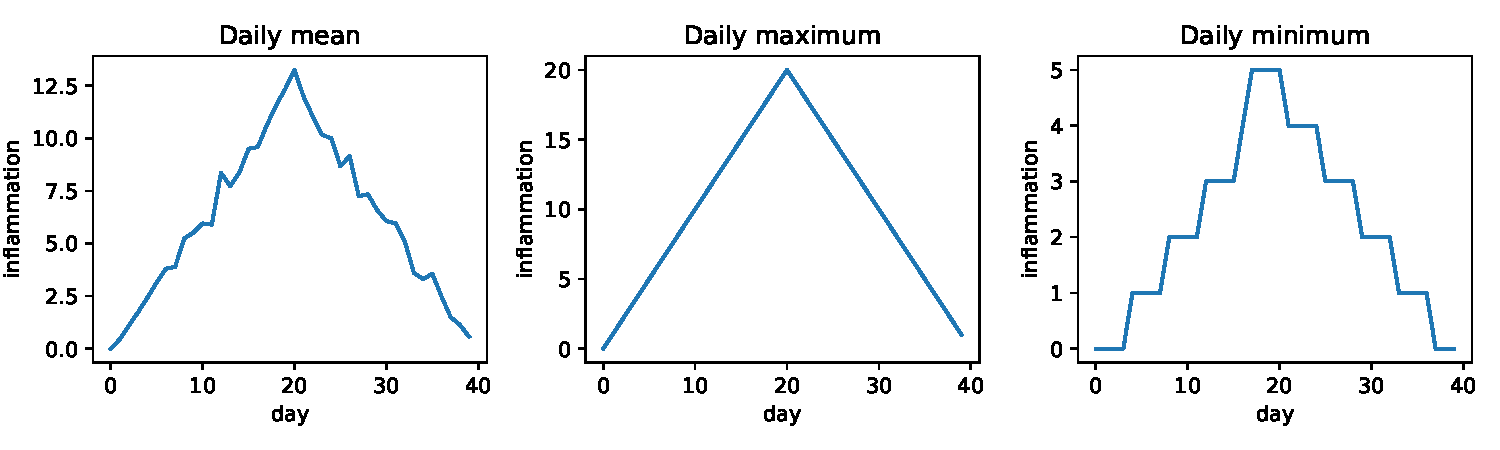
\includegraphics[width=\linewidth]{graphics/inflammation_figure.pdf}

\vspace{-4mm}
\begin{minted}[xleftmargin=6mm,frame=lines,framesep=2mm,linenos,fontsize=\small]{python}
fig = matplotlib.pyplot.figure(figsize=(10.0, 3.0))

axes1 = fig.add_subplot(1, 3, 1); axes1.set_title('Daily mean')
axes1.set_xlabel('day'); axes1.set_ylabel('inflammation')
axes1.plot(numpy.mean(data, axis=0))

axes2 = fig.add_subplot(1, 3, 2); axes2.set_title('Daily maximum')
axes2.set_xlabel('day'); axes2.set_ylabel('inflammation')
axes2.plot(numpy.max(data, axis=0))

axes3 = fig.add_subplot(1, 3, 3); axes3.set_title('Daily minimum')
axes3.set_xlabel('day'); axes3.set_ylabel('inflammation')
axes3.plot(numpy.min(data, axis=0))

fig.tight_layout()
matplotlib.pyplot.savefig('inflammation_figure.pdf')
\end{minted}

Notice that we saved the image as PDF file on line 16. This is exceptionally useful since the resulting PDF file is a vector graphic, not a bitmap. I have actually included this image above - try selecting ``daily maximum'' with your mouse, or try zooming in and seeing how there is no ``pixellation''.

\end{multicols*}
\section{Repeating Actions with Loops}
\begin{multicols*}{2}

Consider the example from the previous section in which we created \mintinline{python}{axes1}, \mintinline{python}{axes2} and \mintinline{python}{axes3} and placed them into a \mintinline{python}{matplotlib} figure. If you look at the code for \mintinline{python}{axes1}, \mintinline{python}{axes2} and \mintinline{python}{axes3} (lines 3 to 5, 7 to 9, and 11 to 13), you'll notice they are all quite similar. The only things that differ for each of these is:

\begin{myitemize}
    \item The third parameter for the \mintinline{python}{fig.add_subplot()} function;
    \item the title of the graph; and,
    \item the data source for the graph.
\end{myitemize}

Everything else about the graphs was the same. This is a great example of when we could use a \textbf{for-loop}. The code sample below \textbf{refactors} \textit{(= rewriting code to make it more elegant, while retaining the same outcome of the code)} the previous code sample to use a for-loop.

\vspace{-4mm}
\begin{minted}[xleftmargin=6mm,frame=lines,framesep=2mm,linenos,fontsize=\small]{python}
fig = matplotlib.pyplot.figure(figsize=(10.0, 3.0))

figure_data = [
    {'title': 'Daily mean',      'numbers': numpy.mean(data, axis=0)}
    , {'title': 'Daily maximum', 'numbers': numpy.max(data, axis=0)}
    , {'title': 'Daily minimum', 'numbers': numpy.min(data, axis=0)}
]

for seqno in range(0, 3):
    this_axes = fig.add_subplot(1, 3, seqno + 1)
    this_axes.set_xlabel('day')
    this_axes.set_ylabel('inflammation')
    this_axes.set_title(figure_data[seqno]['title'])
    this_axes.plot(figure_data[seqno]['numbers'])

fig.tight_layout()
matplotlib.pyplot.savefig('inflammation_figure.pdf')
\end{minted}

\par
A few things to note here:

\begin{myitemize}
    \item Line 1 is the same as it was before.
    \item On lines 3 to 7, we now have a data structure called \mintinline{python}{figure_data}. This is an array with two elements, each of which is in the format \mintinline{python}{{ 'k1': v1, 'k2': v2 }}. This is known as a \textbf{dictionary}. It allows us to store \textbf{values} (e.g. \textit{k1, k2}) for specified \textbf{keys} (e.g. \textit{v1, v2}). So, for example, the value stored at \mintinline{python}{figure_data[0]['title']} is the string \textit{``Daily mean''}.
    \item On lines 9 to 14, we now have a control structure called a \textbf{for-loop}. This means that everything ``inside'' the loop (lines 10-14) is executed in each iteration of the loop. \textbf{In Python, we indicate what is ``inside'' the loop using indentation, which is why lines 10-14 are indented.} This is very important if you are coming from a language like Java where indentation is not as consequential.
    \item On line 9, we define the for-loop using \mintinline{python}{range(0, 3)}. This is a function that generates an array from 0 (inclusive) to 3 (exclusive), i.e., \textit{\{0, 1, 2\}}. The loop iterates across each of these elements, with each iteration storing the element as \mintinline{python}{seqno}. This conveniently means that while we traverse \mintinline{python}{range(0, 3)}, we also traverse the elements of \mintinline{python}{figure_data}, which becomes very useful on lines 13 and 14. It also means, technically, we could have used \mintinline{python}{range(0, len(figure_data))} instead of \mintinline{python}{range(0, 3)}.
    \item However, because \mintinline{python}{fig.add_subplot()} expects \textit{\{1, 2, 3\}} for its third parameter (i.e. 1-indexed instead of 0-indexed), we have the expression \mintinline{python}{seqno + 1} on line 10.
    \item On line 9, we could have alternatively used the expression \mintinline{python}{for seqno, this_value in enumerate(figure_data)}. This would allow us to replace \mintinline{python}{figure_data[seqno]} with simply \mintinline{python}{this_value} on lines 13 and 14. This is similar to a \textbf{for-each loop} (which you may be familiar with if you have a Java background).
\end{myitemize}

You should also know that you can treat a string as an array of one-character strings, and use a for-loop on it likewise:

\vspace{-4mm}
\begin{minted}[xleftmargin=6mm,frame=lines,framesep=2mm,linenos,fontsize=\small]{python}
word = 'oxygen'
for char in word:
    print(char)
\end{minted}

\end{multicols*}

\end{document}